\chapter{Introduction}
\label{cha:introduction}

This chapter presents the overview and general objectives of this thesis.
The first section outlines the background and the concept of
assuring data reliability. Cloud storage availability and integrity challenges
are introduced in the following section. Next, we present the origin of
this work in the context of VPH-Share Cloud Platform. In the final section,
the high-level objectives of this thesis are described.
 
\section{Background and overview}
In the modern world of the 21st century the data and its vast volume
are ubiquitous. The total amount of global data stored to date is estimated
as 4 zettabytes ($4 \times 10^{21}bytes$) in 2013, almost $50\%$ more than in 2012 \cite{idc-data-growth}.
As long as computers spread to 
new domains and new computing paradigms -- as internet of things and big data
-- become a reality, the trend of exponential growth of data volume
will continue. The main sources of data are of various kind:

\begin{itemize}
\item \textbf{personal data} -- generated by and associated with people such as
images, videos, emails, documents etc, stored on privately held devices as
laptops, smartphones or digital cameras as well as by website owners in
big data centers,
\item \textbf{business data} -- generated by companies and corporations
that enables them to run and maintain their daily business,
\item \textbf{experimental data} -- generated by all kind of sensor and
experimental devices from weather stations, to particle accelerators, to
space satellites and stored on academic resources and scientific data centers.
\end{itemize}

It is an engineering challenge to fullfill storage requirements for current
data growth. Nowadays, we observe a rapid shift from privately owned and maintained
computer systems toward virtualized computer infrastructures provided as a service,
namely cloud computing. At least several commercial cloud infrastructure offerings 
provide access to virtualized computer systems at different level -- Infrastructure
as a Service (IaaS), Platform as a Service (PaaS) and Software as a Service (SaaS).
Low costs, high availability and scalability, decent performance degradation and 
seamless integration are often mentioned as major benefits by cloud adopters and
evangelists.\\

Digitalization brought new opportunities and advantages to the business and communities.
As a~result, many of them became strictly tied to their data as a major asset and
can no longer tolerate any data loss. Temporal data unavailability can also pose 
a~problem in domains such as medical care and flight services. With the promise
of scalable data storage, where everything can be stored or archived for future
needs, it is a burning issue to provide means of data loss prevention.\\

In general, the methods of data loss prevention can be divided into two groups:

\begin{enumerate}
\item \textbf{corruption or loss detection} -- that the data content is unavailable
or no longer correct,
\item \textbf{corruption or loss recovery} -- that after data corruption detection
we can recover its original properties of availability and integrity.
\end{enumerate}

A number of methods exist and are in widespread use nowadays. Storage hardware
solutions -- CDs, hard disks, etc -- utilize error correcting codes (ECC) to prevent
small scale errors on read/write operations. Network protocols and software packages
distribution use hash-based checksums to verify the integrity of the content. Data
backups and replication are universal way of enabling recovery from data loss.\\

Ideally, from the user point of view, data storage solution should provide highly
available and fault-tolerant access to the data and be free of data corruption and
unavailability problems. However, it often appears that the above-mentioned
criteria cannot be met in practice,
especially when relying on single service provider. Cloud service providers protect
their customers data with data replication to geographically distributed zones,
strong securitiy policies and infrastructure monitoring. Even though, recently
a~number of cloud failures occured, questioning the reliability of
cloud solutions. Malicious and accidental data corruption threats also require
attention.\\ 

The standard concept of checking data integrity is based on checksum verification.
It consists of two major steps -- initial setup and verification. The first step
concerns with initial data deployment and computing checksum metadata of the content
-- a hash.In the verification step the integrity checksums of the data are once more
computed and compared with the reference ones. In the scope of this thesis, we discuss
the means of providing data reliability, by which we mean both:

\begin{enumerate}
\item \textbf{availability} -- that the data is available to the requesting entity,
\item \textbf{integrity} -- that the data remains untouched by malicious or undesired
modifications.
\end{enumerate}

Managing data availability and integrity of data in cloud storage environment is the
subject of this thesis. As we mentioned above, to provide a solid way of assuring data
reliability we must address both data corruption detection and recovery. The idea is
to, apart from the internal cloud provider replication, replicate the data over multiple
cloud provider resources, continuously monitor its integrity and enable possibility to restore corrupted
entities from existing replicas. In case of irreparable corruption we should notify the
owner about the data problem. Replicating the data over cloud providers will build another
abstraction layer on top of cloud service and will allow to use them interchangeably in so
called federation of cloud storage. With federated approach we can easily detect cloud provider
failure and switch to another.

\section{Cloud storage data reliability challenges}

Over the last years, we observe a rapid shift from privately owned and maintained
storage resources toward cloud storage solutions. The cloud model of business become
popular and adopted by many organizations. The main driving forces of cloud computing
shift are low costs, high availability and scalability, decent performance degradation
and seamless integration. While the emerging trend determines a significant step forward 
in storage technology and brings a lot of advantages as data replication, no administration
costs, pay-as-you-use, SLA contracts -- it can appear challenging for ensuring data 
reliability. Remotely available resources introduce network transfer rates and latency issues,
while SLA contracts are mostly best-effort -- cloud provider will not charge fees if service
quality has not been met. Additionally, recent cloud storage failures or security break
reports shown that we cannot entrust our data to cloud providers entirely.\\
 
Classic checksum-based integrity verification methods are based on the whole content of data. It
poses a challenge to efficiently verify the integrity of vast volumes of data stored on remote resources,
where network transfer rates and latency comes into play. Additionally, cloud
storage providers charge fees not only for storage space used, but also for storage transfer.
Consequently, cloud storage data reliability methods should take these limitations into
consideration. It appears inevitable that cloud storage data integrity can be only provided with
some level of probability and has to be based on a fraction of the file. A part of this thesis main
objective is to select and implement a network-efficient method of ensuring data reliability.


\section{VPH-Share Cloud Platform context}
This thesis originates as a part of the VPH-Share project founded by European Commission
which brings together twenty international partners from academia, industry and healthcare,
led by University of Sheffield. Its main goal is to build a collaborative computing
environment and infrastructure where researchers from the domain of physiopathology of
the human body will work together on developing new medical simulation software. The inspiring
vision is to create a versatile environment for sharing of information -- tools, models and data
-- to work efficiently towards building a complete model of the human body.\\

The project has layered architecture divided into work packages distributed among consortium
members (see figure \ref{fig:dri-high-level}). The design is based on cloud computing middleware
-- a hybrid of commercial and private resources on top of hardware layer. Data and Compute
Cloud Platform is one of the main building blocks of the VPH-Share project. Its goal is to
develop and integrate a consistent service-based cloud infrastructure that will enable VPH
community to deploy basic components of VPH-Share application workflows (known as Atomic Services)
on the available computing resources and then enact workflows using these services. Access to the
services layer will be provided to system users through user interface(UI).

\begin{figure}[h!]
	\centering
	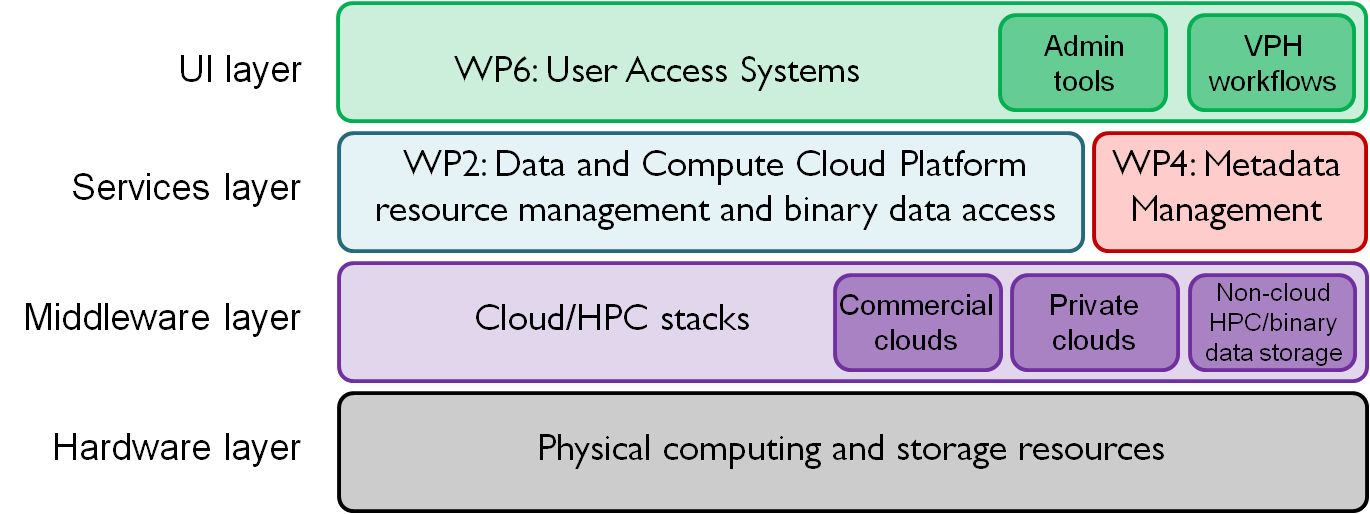
\includegraphics[width=0.8\textwidth]{images/vph-high-level.png}
	\caption{VPH-Share overview\\
	The project aims to build a collaborative computing environment
	for researchers of human body to work on developing new medical simulation software.
	Its design has layered architecture centered around service-based Data and Compute
	Cloud Platform built on top of hybrid cloud middleware, both commercial and private. The VPH-Share
	users use the platform through common user interface layer.}
	\label{fig:dri-high-level}
\end{figure} 


VPH-Share specifies three groups of users:
application providers, domain scientists and system administrators. Application providers
are responsible for developing and installing scientific applications and software packages.
Domain scientists are actual researchers of VPH community who will use and benefit from 
the platform. Finally, system administrators is a group of priviledged users who will
manage platform's hardware resources and will administer and maintain it.\\

According to the platform's design, data will be stored on federated cloud storage resources --
both commercial and private -- and available via common access layer. It is foreseen that stored
data volumes will be significant, but predominantly of static nature -- upon upload its content will
remain untouched. Additional measures should ensure data availability and integrity.As a result, two
of the key project's requirements regarding data storage and integrity are:

\begin{itemize}
\item \textbf{access to large binary data in the cloud} -- specified groups of users will
be able to query for and store binary data uploaded or generated by workflows within the platform, 
\item \textbf{data reliability and integrity} -- platform users will be able to tag datasets
for automatic availability and integrity monitoring, set validation and replication policies,
as well as receive notifications about data integrity violations.
\end{itemize}


\section{Objectives of this work}

As it was mentioned in the previous sections, there is a~need for creation of a~service that
will provide monitoring of data reliability and integrity (DRI) in federation of cloud storage
resources, in particular within VPH-Share Cloud Platform environment. The high-level objective of this
thesis is to design and implement such service that:

\begin{enumerate}
\item efficiently and  periodically monitor the integrity of the federated cloud storage,
\item notify the user about discovered data corruption in advance of data retrieval, 
\item provide possibility to restore corrupted data from replicas in other cloud providers.
\end{enumerate}

In this thesis, by efficient data integrity validation we mean network efficiency. Our goal is to minimize network
traffic required to validate a~file, while still be able to detect corruption on acceptable
level of probability.\\


\begin{figure}[h!]
	\centering
	\includegraphics[width=0.8\textwidth]{images/DRI-objectives.png}
	\caption{DRI service is a~stateless web service within service-based VPH-Share Cloud Platform.
	Its main objective is periodical validation of data availability and integrity stored on
	federated cloud storage. All the integrity metadata is stored in metadata registry, while data access
	is perfomed via common federated cloud storage access layer to multiple cloud providers. Corruption
	or unavailability violations are sent to the user via Notification Service component.}
	\label{fig:dri-objectives}
\end{figure} 

At this point, the architecture of DRI service can be presented as a separate component within service-based 
environment that depends on other VPH-Share Cloud Platform core components visible in figure \ref{fig:dri-objectives}.
Conceptually, DRI service is a part of service-based VPH Cloud Platform architecture and provides
a~stateless web interface that enables managing data reliability (see figure \ref{fig:dri-objectives}).
To fullfill its responsibilities
DRI depends on a~number of other services. All of the service metadata regarding integrity checksums
and statuses, replication policies and federated cloud access is stored externally in metadata registry.
Data integrity and replication is performed on a~multiple cloud providers via common federated cloud
storage access layer. User notifcations are sent via external notification service.\\

DRI considers a~concept of dataset -- simply a set of files. Upon tagging dataset as managed DRI triggers
integrity checksums computation and stores them in metadata registry. As long as dataset remains managed
a~periodical availability and integrity verification takes place. When data corruption is detected the
user is notified about the errors via notification service and can restore the content from other replicas.


